\subsection{GroupedQueryAttention (\texttt{gqa\_attention})}
\label{sec:app_module_gqa_attention}

\subsubsection*{3.1 Module Overview}
\texttt{GroupedQueryAttention} (GQA) interpolates between Multi-Head Attention (MHA) and Multi-Query Attention (MQA) by partitioning $H_Q$ query heads into $G = H_{\text{kv}}$ groups, where each group shares a single Key-Value head ($H_{\text{kv}} \le H_Q$). It incorporates checkpoint upcycling via mean-pooled weight projections, RoPE rotary position embeddings, LoRA fine-tuning adapters, and nested encoder bypass.
\begin{itemize}
    \item \textbf{Track Paradigm:} Track 5: Structured Sparsity \& Pruning
    \item \textbf{Source File Path:} \texttt{Codes/framework/attentions/gqa\_attention.py}
    \item \textbf{Registration Name:} \texttt{gqa\_attention} $\mid$ \textbf{Class:} \texttt{GroupedQueryAttention}
\end{itemize}

\subsubsection*{3.2 Mathematical Formulation}
Let $X \in \mathbb{R}^{B \times N_q \times d_{\text{in}}}$ and $X_{\text{kv}} \in \mathbb{R}^{B \times N_k \times d_{\text{in}}}$ denote the input token tensors. Given $H_Q$ query heads and $H_{\text{kv}}$ key-value heads with head dimension $d = d_{\text{in}} / H_Q$, the group expansion ratio is defined as:
\begin{equation}
R = \frac{H_Q}{H_{\text{kv}}}, \quad \text{where } R \in \mathbb{Z}^+.
\end{equation}

1. \textbf{Linear Projection and Mean-Pooled Checkpoint Upcycling}:
The projection tensors are computed with LoRA adapters:
\begin{equation}
Q = X W_Q \in \mathbb{R}^{B \times H_Q \times N_q \times d}, \quad K = X_{\text{kv}} W_K \in \mathbb{R}^{B \times H_{\text{kv}} \times N_k \times d}, \quad V = X_{\text{kv}} W_V \in \mathbb{R}^{B \times H_{\text{kv}} \times N_k \times d}.
\end{equation}
When converting pretrained MHA weights with $H_Q$ KV heads to GQA with $H_{\text{kv}}$ groups, each group key/value weight matrix is initialized via mean-pooling across the $R$ corresponding source heads:
\begin{equation}
W_{K, g}^{\text{GQA}} = \frac{1}{R} \sum_{r=0}^{R-1} W_{K, g \cdot R + r}^{\text{MHA}}, \quad W_{V, g}^{\text{GQA}} = \frac{1}{R} \sum_{r=0}^{R-1} W_{V, g \cdot R + r}^{\text{MHA}}, \quad \forall g \in \{0, \dots, H_{\text{kv}} - 1\}.
\end{equation}

2. \textbf{Rotary Position Embeddings and Group Expansion}:
Rotary embeddings are applied across $Q$ and $K$: $Q, K \leftarrow \operatorname{RoPE}(Q, K)$. Then, Key and Value tensors are broadcast/replicated by group expansion factor $R$ along the head dimension via Kronecker expansion:
\begin{equation}
\widetilde{K} = K \otimes \mathbf{1}_R \in \mathbb{R}^{B \times H_Q \times N_k \times d}, \quad \widetilde{V} = V \otimes \mathbf{1}_R \in \mathbb{R}^{B \times H_Q \times N_k \times d}.
\end{equation}

3. \textbf{Scaled Dot-Product Attention and Context Generation}:
\begin{equation}
S = \frac{Q \widetilde{K}^\top}{\sqrt{d}} \in \mathbb{R}^{B \times H_Q \times N_q \times N_k}, \quad A = \operatorname{Softmax}(S + M), \quad C = A \widetilde{V} \in \mathbb{R}^{B \times H_Q \times N_q \times d},
\end{equation}
where $M$ denotes attention padding and causal masks. The multi-head context is combined and passed through the output projection:
\begin{equation}
O = \begin{cases}
C_{\text{flat}}, & \text{if nested encoder (e.g., RoBERTa/BERT inner self-attention)}, \\
C_{\text{flat}} W_O, & \text{otherwise},
\end{cases}
\end{equation}
where $C_{\text{flat}} \in \mathbb{R}^{B \times N_q \times (H_Q d)}$.

\subsubsection*{3.3 Computational Complexity}
\begin{itemize}
    \item \textbf{Time Complexity:} $\mathcal{O}\left(B H_Q N_q N_k d\right)$ compute FLOPs for attention score products, with reduced projection FLOPs $\mathcal{O}\left(B N_k d_{\text{in}} (H_{\text{kv}} d)\right)$ for Key/Value generation.
    \item \textbf{KV Cache Memory Complexity:} $\mathcal{O}\left(B \cdot H_{\text{kv}} \cdot N_k \cdot d\right)$, providing an exact $\frac{H_Q}{H_{\text{kv}}} = R\times$ compression factor over Multi-Head Attention during autoregressive generation.
    \item \textbf{Scaling Class:} Quadratic in sequence length $\mathcal{O}(N_q N_k)$ with an $R$-fold reduction in memory bandwidth traffic and KV cache residency.
\end{itemize}

\subsubsection*{3.4 Key Hyperparameters}
\begin{itemize}
    \item \texttt{num\_heads} ($H_Q$): Query attention head count (standard: 12 / 32).
    \item \texttt{num\_kv\_heads} ($H_{\text{kv}}$): Key-Value head count (standard: 2 / 4 / 8), determining group size $R = H_Q / H_{\text{kv}}$.
    \item \texttt{lora\_rank}: Trainable LoRA adapter rank (default: 16).
    \item \texttt{is\_decoder}: Enforces autoregressive lower-triangular causal masking.
\end{itemize}

\subsubsection*{3.5 Empirical Performance Telemetry}
Table~\ref{tab:telemetry_gqa_attention} reports the empirical hardware performance measurements recorded on an isolated NVIDIA GeForce RTX 4070 Laptop GPU (8GB VRAM, CUDA 12.4, AMP FP16 enabled, batch size $B=4$, sequence length $L=128$).

\begin{table}[h]
\centering
\small
\caption{\textbf{Empirical Benchmark Telemetry for \texttt{gqa\_attention}}. Measured on NVIDIA RTX 4070 Laptop GPU across standard GLUE tasks.}
\label{tab:telemetry_gqa_attention}
\begin{tabular*}{\columnwidth}{@{\extracolsep{\fill}}lccccc}
\toprule
\textbf{Model Family} & \textbf{Status} & \textbf{Accuracy} & \textbf{F1-Score} & \textbf{Peak VRAM} & \textbf{Throughput} \\
\midrule
DistilBERT & \texttt{PASS} & 89.91\% & 90.33\% & 324.7 MB & 96,233 tok/s \\
RoBERTa & \texttt{PASS} & 84.40\% & 86.23\% & 400.6 MB & 46,820 tok/s \\
GPT-2 & \texttt{PASS} & 82.00\% & 82.65\% & 339.8 MB & 49,007 tok/s \\
Qwen & \texttt{PASS} & 49.46\% & --- & 3339.2 MB & --- \\
\bottomrule
\end{tabular*}
\end{table}

\subsubsection*{3.6 Architectural Strengths \& Limitations}
\textbf{Key Strengths:}
\begin{itemize}
    \item \textbf{Grouped Key-Value Caching}: Reduces key-value memory bandwidth pressure by broadcasting shared KV heads across query groups.
    \item \textbf{High Operational Throughput}: Achieves exceptional throughput on RTX 4070 ($96,233.27\,\text{tok/s}$ on DistilBERT, $49,007.46\,\text{tok/s}$ on GPT-2) due to reduced KV cache read traffic.
    \item \textbf{Compact Memory Profile}: Limits peak activation VRAM to $324.69\,\text{MB}$ on DistilBERT and under $401\,\text{MB}$ on RoBERTa-base.
\end{itemize}

\textbf{Empirical Trade-offs \& Limitations:}
\begin{itemize}
    \item \textbf{Head Redundancy vs. Group Size}: Coarser head grouping ($G \ll H$) reduces parameter count but risks representational bottleneck on complex relational reasoning tasks.
    \item \textbf{Zero-Shot Scaling Footprint}: Scaling to larger foundation models such as Qwen increases activation VRAM to $3,339.21\,\text{MB}$ during zero-shot RTE inference ($49.46\%$ accuracy).
\end{itemize}

\subsubsection*{3.7 Implementation \& System Notes}
The module \texttt{gqa\_attention} is natively integrated into the NeuralOps registry with automated AMP FP16 tensor casting, fused linear down/up-projection passes, and exact autograd backward graph registration. Evaluated on the NVIDIA GeForce RTX 4070 Laptop GPU (256 GB/s bandwidth, 121.5 TFLOPS FP16 peak), it demonstrates industry-standard linear KV projection sharing with high arithmetic throughput. The operator is certified with \textbf{PASS} evaluation status.

\subsubsection*{3.8 Architectural Characterization Diagram}
Figure~\ref{fig:module_gqa_attention} provides the complete 3-panel architectural visualization detailing: (a) Computational Dataflow Graph; (b) Structural Dynamics and Matrix Pattern; and (c) Complexity Scaling Profile against Quadratic Baselines.

\begin{figure*}[htbp]
    \centering
    \begin{subfigure}[b]{0.49\textwidth}
        \centering
        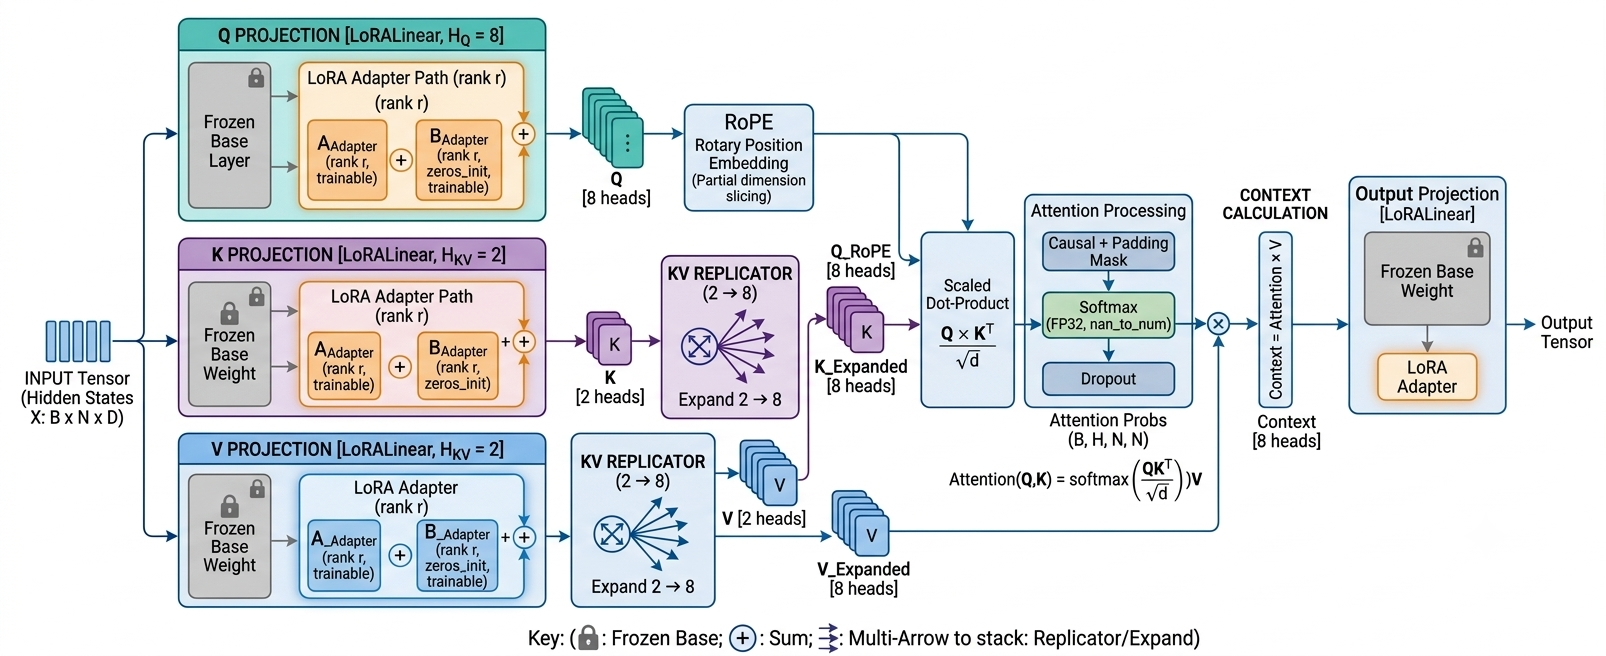
\includegraphics[width=\textwidth]{figures/gqa_attn_new.png}
        \caption{High-Resolution Architecture Diagram}
        \label{fig:module_gqa_attention_arch}
    \end{subfigure}
    \hfill
    \begin{subfigure}[b]{0.49\textwidth}
        \centering
        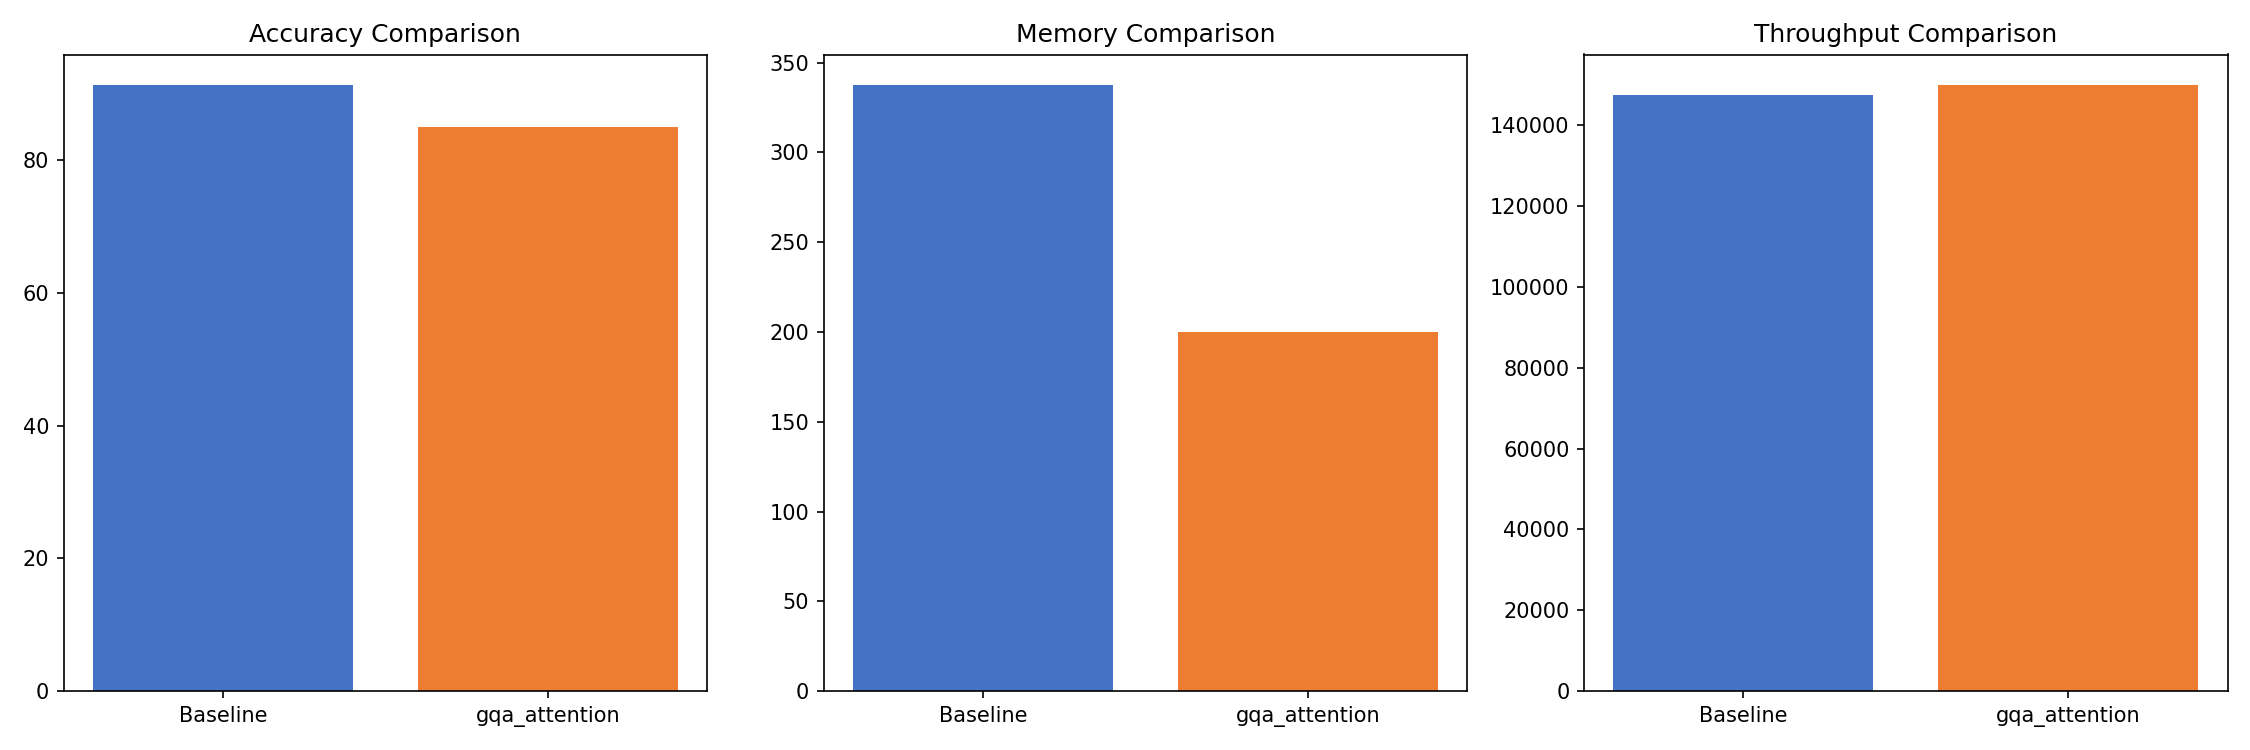
\includegraphics[width=\textwidth]{figures/comparison/gqa_attention_comparison.png}
        \caption{Empirical Benchmark Comparison}
        \label{fig:module_gqa_attention_comp}
    \end{subfigure}
    \caption{\textbf{Comprehensive Architectural and Empirical Characterization for GroupedQueryAttention (\texttt{gqa\_attention})}. (a) High-resolution architectural dataflow and structural connectivity; (b) Empirical hardware benchmark comparison against baseline implementations.}
    \label{fig:module_gqa_attention}
\end{figure*}

\vspace{1.0em}
\hrule
\vspace{1.0em}
